\subsection{Wydajność ALL(*) ze względu na języki}
\begin{figure}[h]
\begin{tabular}{|l||r|}
\hline
Grammar & KB/sec \\
\hline\hline
XML & 45'993 \\
Java & 24'972 \\
JSON & 17'696 \\
DOT & 16'152 \\
Lua & 5'698 \\
C & 4'238 \\
Verilog2001 & 1'994 \\
Erlang &751 \\
\hline
\end{tabular}
\caption{Wydajność w
KByte/sec. Lexing+parsing;
cały wejście załadowane do RAM.}
\end{figure}

\begin{figure}[h]
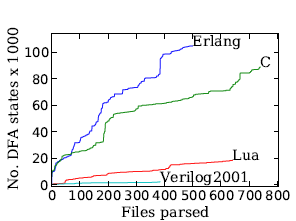
\includegraphics[scale=0.8]{Figure12.png}
\caption{
Tempo wzrostu DFA vs ilość parsowanych plików.
Pliki parsowane w kolejności w jakiej były na dysku.
}
\end{figure}

Obrazek 11 podaje wydajność w bajtach na sekundę wszystkich parserów ALL(*)
dla 8 języków włączając w to Javę dla porównania. Ilość plików testowych
i rozmiary plików różnią się znacznie (według wejścia które mogliśmy rozsądnie zebrać);
mniejsze pliki uzyskują wyższą wariancję czasu parsowania.
\begin{itemize}
\item C Pochodzi ze specyfikacji C11; nie ma pośredniej lewej rekursji,
zmieniona reguła wrażliwa na stos aby  wykonać SLL (zobacz tekst poniżej): 813
preprocesowanych plików, 159.8M źródeł z bazy postgres.
\item Verilog2001 Pochodzi z specyfikacji Verilog 2001, usunięta pośrednia lewa rekursja:
385 plików, 659k z [3] i internetu.
\item JSON Pochodzi ze specyfikacji. 4 pliki, 331k z twittera.
\item DOT: Pochodzi ze specyfikacji. 48 plików,19.5M zebranych z internetu.
\item Lua: Pochodzi ze specyfikacji Lua 5.2. 751 plików, 123k z githuba.
\item XML Pochodzi ze specyfikacji. 1 plik, 117M z XML benchmark.
\item Erlang Pochodzi z gramatyki LALR(1). 500 preprocesowanych plików, 8M.
\end{itemize}
Niektóre z tych gramatyk mają wydajność rozsądną ale dużo wolniejszy czas parsowania w
porównaniu do Javy i XML ale demonstrują że programiści mogą konwertować język
specyfikacji do ANTLR meta-składni
i dostać działającą gramatykę bez dużej modyfikacji.
(W naszym doświadczeniu specyfikacje gramatyki są rzadko dostrajane do szczeólnych narzędzi lub strategii parsowania i są często niejednoznaczne.) Później, programiści mogą użyć profilowania ANTLR i diagnostyki do polepszenia wydajności tak jak inne programistyczne zadanie.
Dla przykładu, specyfikacja gramatyki C11 jest LL nie SLL
z powodu reguły declarationSpecifiers, która zmieniliśmy aby była SLL w naszej gramatyce C (dostając 7x przeypieszenia prędkości).
